% The paper on using Luau telemetry to measure the effectiveness of type error reporting.

\documentclass[
  acmsmall,
  review,
  anonymous,
]{acmart}

%\settopmatter{printfolios=true,printccs=false,printacmref=false}

\overfullrule=1mm
\citestyle{acmauthoryear}
%\setcitestyle{round}

\usepackage{alltt}
% \usepackage{amssymb} -- already loaded by acmart
\usepackage{calc}
\usepackage{cleveref}
\usepackage{listings}
\usepackage{mathpartir}
\usepackage{pifont}
\usepackage{siunitx}
\usepackage{tikz}
\usepackage{wasysym}
\usepackage{wrapfig}
\usepackage{xcolor}
\usetikzlibrary{shapes.geometric}

\begin{document}

\title{Millions of Type Errors}
\subtitle{Impersonal Telemetry to Measure User Experience}
% lean, lite, modest, non-intrusive, private, ...

% Alphabetical order for authors?

\author{Ben Greenman}
\orcid{0000-0001-7078-9287}
\affiliation{%
  \institution{Brown University}
  \city{Providence}
  \state{Rhode Island}
  \country{USA}
}
\email{benjaminlgreenman@gmail.com}

\author{Alan Jeffrey}
\orcid{0000-0001-6342-0318}
\affiliation{%
  \institution{Roblox}
  \city{San Mateo}
  \state{California}
  \country{USA}
}
\email{ajeffrey@roblox.com}

\author{Shriram Krishnamurthi}
\orcid{0000-0001-5184-1975}
\affiliation{%
  \institution{Brown University}
  \city{Providence}
  \state{Rhode Island}
  \country{USA}
}
\email{shriram@brown.edu}

\author{Mitesh Shah}
\orcid{TODO}
\affiliation{%
  \institution{Roblox}
  \city{San Mateo}
  \state{California}
  \country{USA}
}
\email{mshah@roblox.com}

%\renewcommand{\shortauthors}{...}

%%
%% The abstract is a short summary of the work to be presented in the
%% article.
\begin{abstract}
  \anon{Roblox Studio} is a tool which places programming in the hands of
  millions of creators, ranging from high school students to professional
  development studios. It has the ability to report telemetry data,
  which allows large-scale measurement of the creator experience. In
  this paper, we discuss one use of telemetry, to measure the experience
  of type error reporting.
\end{abstract}

\newcommand{\code}[1]{\texttt{#1}}
\newcommand{\FILL}{\textbf{FILL}}
\newcommand{\dotscale}[1]{\scalebox{0.72}{#1}}
\newcommand{\wideas}[2]{\makebox[\widthof{#2}][l]{#1}}
\newcommand{\twoline}[2]{\parbox[s]{1.4cm}{\flushleft#1\newline#2}}
\newcommand{\chkYes}{\dotscale{\CIRCLE}}
\newcommand{\chkMaybe}{\wideas{\dotscale{\Circle}}{\chkYes}}
\newcommand{\chkNo}{\wideas{}{\chkYes}}
\newcommand{\pct}[1]{\SI{#1}{\percent}}
\newcommand{\modefont}[1]{\texttt{#1}}
\newcommand{\mnocheck}{\modefont{nocheck}}
\newcommand{\mnonstrict}{\modefont{nonstrict}}
\newcommand{\mstrict}{\modefont{strict}}

%%
%% The code below is generated by the tool at http://dl.acm.org/ccs.cfm.
%% Please copy and paste the code instead of the example below.

\begin{CCSXML}
<ccs2012>
<concept>
<concept_id>10011007.10011006.10011039.10011311</concept_id>
<concept_desc>Software and its engineering~Semantics</concept_desc>
<concept_significance>500</concept_significance>
</concept>
<concept>
<concept_id>10011007.10011006.10011008.10011024.10011032</concept_id>
<concept_desc>Software and its engineering~Constraints</concept_desc>
<concept_significance>100</concept_significance>
</concept>
<concept>
<concept_id>10011007.10011006.10011008.10011009.10011012</concept_id>
<concept_desc>Software and its engineering~Functional languages</concept_desc>
<concept_significance>100</concept_significance>
</concept>
</ccs2012>
\end{CCSXML}

\ccsdesc[500]{Software and its engineering~Semantics}
\ccsdesc[100]{Software and its engineering~Constraints}
\ccsdesc[100]{Software and its engineering~Functional languages}

\keywords{types, gradual typing, telemetry, user study, large-scale study}

\maketitle

\section{Introduction}
\label{s:introduction}

\anon{Roblox} is a platform for \anon{shared virtual experiences},
with 56~million Daily Active Users, and 49~billion hours of engagement in
2022~\anon[(ANONYMIZED CITATION)]{\cite{roblox-quarterly-results}}.
There are \textbf{XX}~million creators using \anon{Roblox Studio},
and \textbf{YY}~million creations.

\anon{Roblox experiences} are scripted using the 
\anon{Luau} programming language~\anon[(ANONYMIZED CITATION)]{\cite{luau-lang.org}},
an extension of \anon{Lua~5.1~\cite{lua}}.
The main extension is the addition of a static type system, which uses
type inference to synthesize types for user code. These types
are used primarily in type-driven tooling such as autocomplete
and API documentation~\anon[(ANONYMIZED CITATION)]{\cite{luau-autocomplete}},
but creators can also opt in to receiving type error reports.

As discussed in~\anon[(ANONYMIZED CITATION)]{\cite{bfj-hatra-2021}},
the goals of the \anon{Luau} type system are rather different from
a traditional type system, which focuses on compilation and memory safety.
\anon{Luau} has a very heterogeneous user community, ranging from
students in code camps to professional development studios. These
creators have quite different needs, with different emphases on
enabling rapid creation and ensuring software quality.

In this paper, we investigate methods for measuring the effectiveness
of the \anon{Luau} type system in development of \anon{Roblox} scripts.
In comparison to prior work~(\cref{s:related}), which is either small in scale
or depends on personally identifiable information~(PII),
we performed a large-scale study using pseudonymized \emph{telemetry}.

\anon{Roblox Studio} has a telemetry system, which is used to gauge
the effectiveness of creation features. This system stochastically
determines which sessions should report telemetry, and for those
sessions, reports telemetry records back with a summary of the
session. In the case of this study, the telemetry includes data on the
number of errors at various levels of granularity: in the current edit
region, in the current file, and in every file which was type
checked.

The telemetry data we analyzed does not contain any PII:
no source code;
no source code locations;
no error messages (which may contain source code);
no record of the creator's identity, locale, or IP address;
and no information about what creation the data came from.
Telemetry records are correlated by session, using a pseudonymized
session identifier.

Most users of \anon{Roblox Studio} do not opt in to type error
reporting, and so they do not see the ``squiggly underlining'' that
indicates a type error site. Nonetheless, the type inference system
still runs (since it drives autocomplete and other type-based tools) and
so we can record which type errors would have been reported had the
user enabled type error reporting. As a result, we can investigate
which type errors are  fixed by users, even if they did not opt in to
type error reporting.

With this telemetry data, we investigate research questions about
the adoption and benefits of type analysis.
First, to learn how many creators use type analysis of any sort
and to estimate whether they pay attention to the results (\FILL{} really, attention?).
Once in type-analysis mode, do creators stay, or revert to no-check?
Second, what errors do creators face and how do they respond.
Are the error highlights helpful for removing the error?
Is there any indication that type analysis improves the quality of the development experience?

This paper is the first to use telemetry as a mechanism for
large-scale measurement of the effectiveness of type error reporting.
Our data captures \textbf{XX} sessions, for a total of \textbf{YY}
hours and \textbf{ZZ} type errors.

Telemetry cannot replace user studies, as there is no way to measure
creator sentiment, but provide complementary data at scale.

\paragraph{Contributions}
\begin{itemize}
  \item
    Design of a low-overhead, (black-box / PII-safe / impersonal)
    telemetry method, that other
    researchers can build on.

  \item
    Lessons from millions of type errors about
    the adoption of strict type analysis,
    the usefulness of type errors,
    and \FILL{}.
    These findings are especially important for the
    gradual typing, success typing, and semantic subtyping communities.

  \item
    \FILL{} any surprises when doing the analysis?
    Note, no ML for analysis, we do not have a corpus of text.

\end{itemize}

Analysis pipeline to be freely available.
Data may be available, depends on Roblox.


\section{\anon{Roblox} Context}
% https://create.roblox.com/docs/scripting/luau

FILL table = object

\begin{figure}

  \makeatletter
  \if@ACM@anonymous
    
\includegraphics[width=.45\textwidth]{img/anon-studio.png}
    
\includegraphics[width=.45\textwidth]{img/anon-studio-ide.png}
  \else
    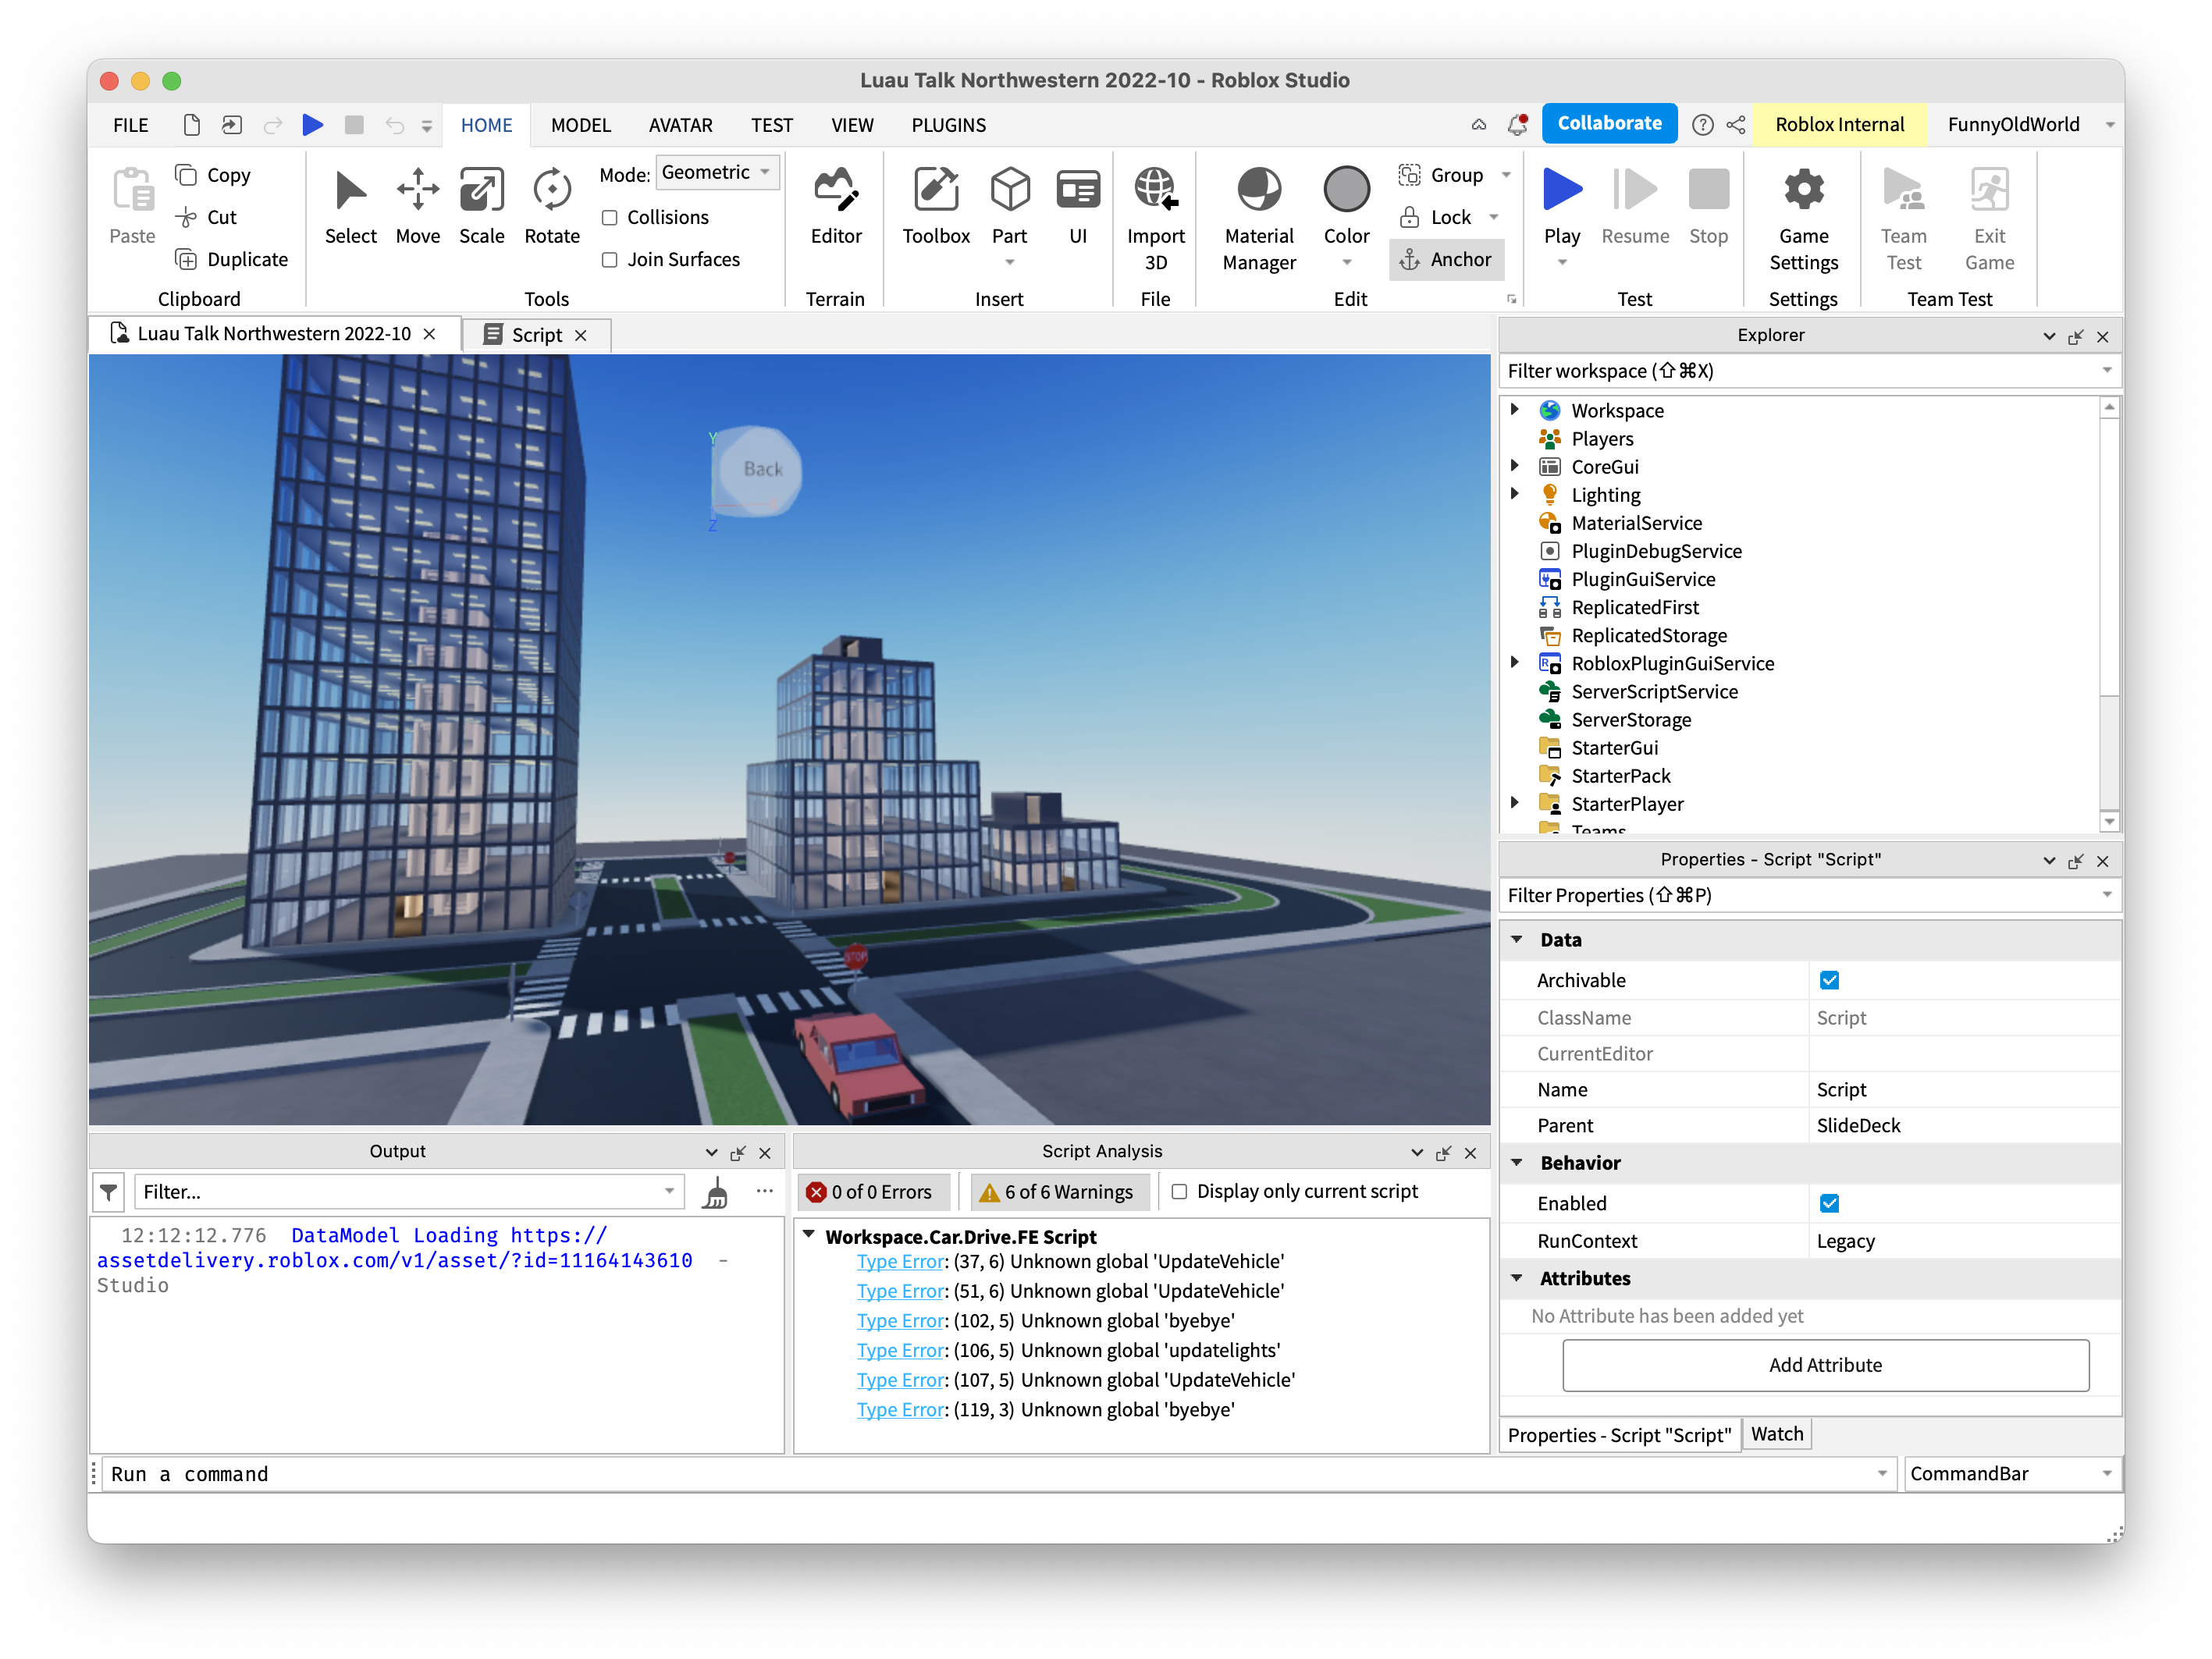
\includegraphics[width=.45\textwidth]{img/roblox-studio.png}
    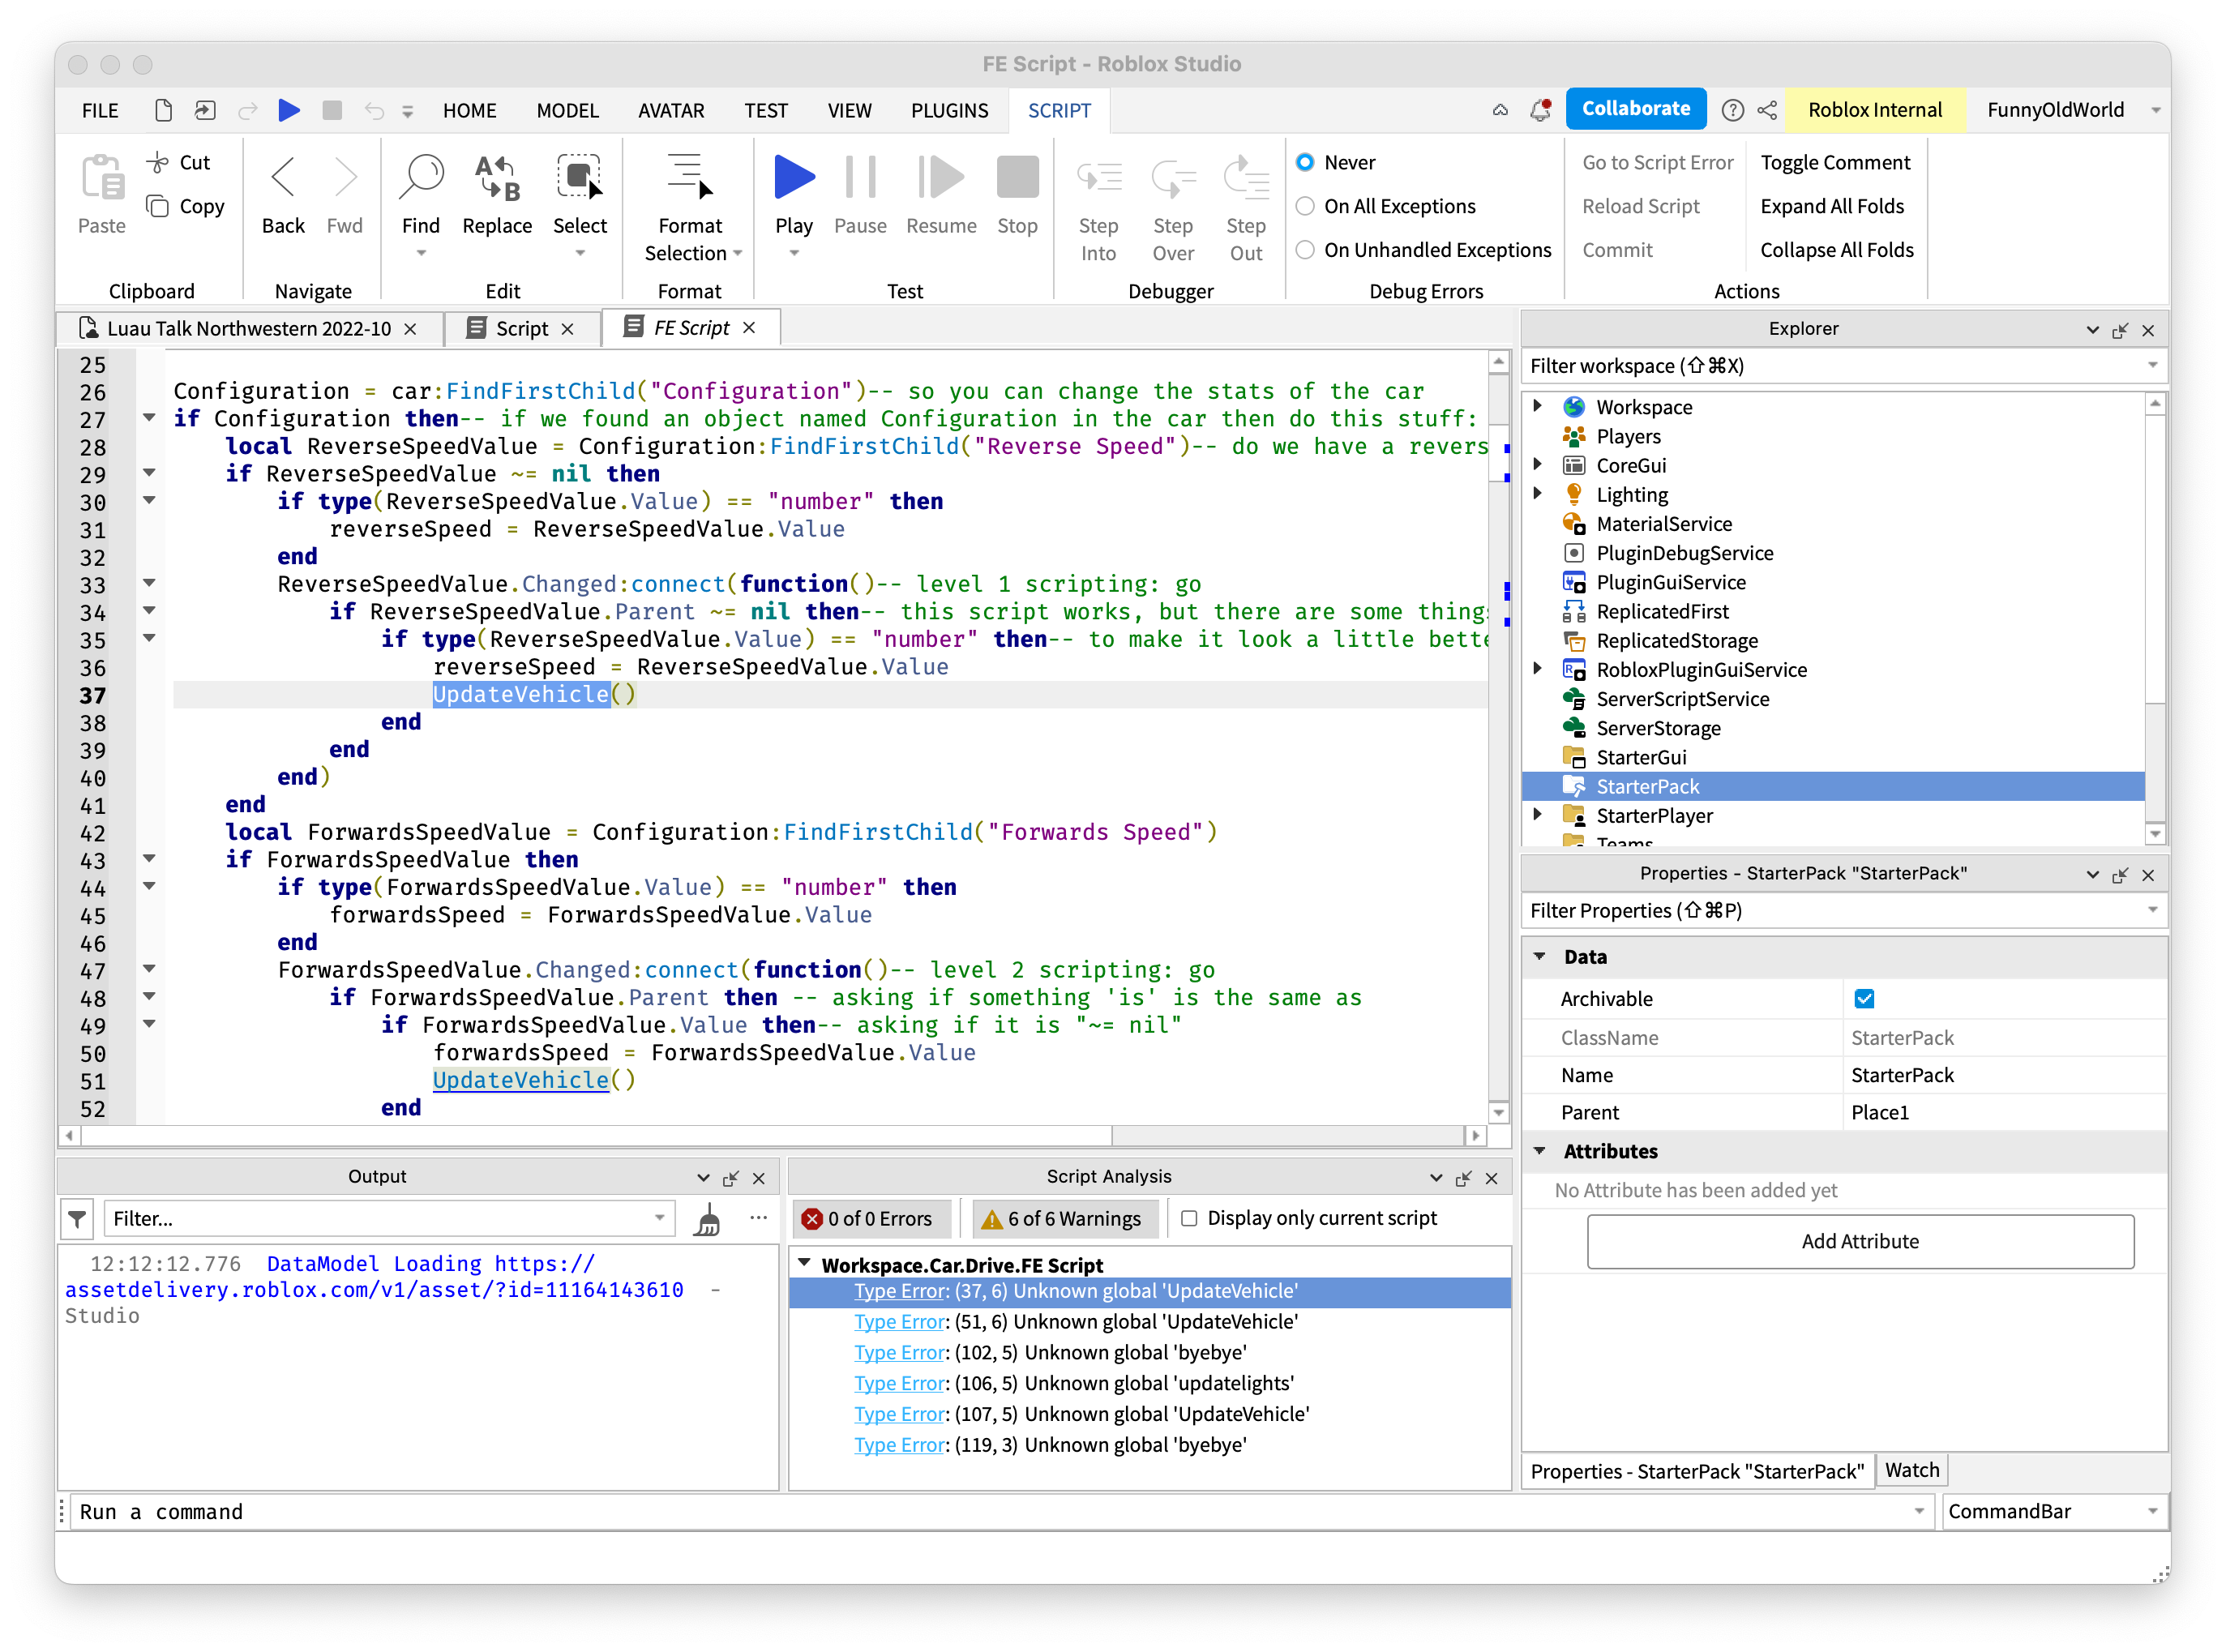
\includegraphics[width=.45\textwidth]{img/roblox-studio-ide.png}
  \fi
  \makeatother

  \caption{\anon{Roblox Studio 3D creation} tools (left) and IDE (right)}
  \label{fig:roblox-studio}
\end{figure}
      
Creators of \anon{Roblox experiences} use \anon{Roblox Studio},
which combines \anon{3D creation} tools as well as an Integrated
Developer Environment (IDE), as seen in Fig.~\ref{fig:roblox-studio}.
The IDE includes an optional ``Script Analysis'' widget, which
reports syntax errors, type errors, and problems identified by
lint tools. The script editor also (optionally) highlights
the location in code where reported errors occur.

To opt in to type error reporting, creators set a \emph{mode}
for each script, which is one of:
\begin{itemize}
  \item \mnocheck{}: only syntax errors are reported,
  \item \mnonstrict{}: all syntax errors, and a subset of ``high probability'' type errors, are reported, or
  \item \mstrict{}: all syntax errors and type errors, are reported.
\end{itemize}
As an example of nonstrict mode, the following program only reports one error:
\begin{verbatim}
--!nonstrict
local x = { p = 5, q = nil }
if condition then x.q = 7 end
local y = x.p + x.q --> no type error
local z = x.r       --> "Key 'r' not found in table 'x'"
\end{verbatim}
but in strict mode it reports two:
\begin{verbatim}
--!strict
local x = { p = 5, q = nil }
if condition then x.q = 7 end
local y = x.p + x.q --> "Type 'nil' could not be converted into 'number'"
local z = x.r       --> "Key 'r' not found in table 'x'"
\end{verbatim}
In cases like this, where it is undecidable whether there will be a run-time error,
strict mode errs on the side of reporting an error, and nonstrict mode errs on
the side of suppressing the error.

Both modes report the \verb|Key 'r' not found in table 'x'| error --
misspellings of property names are common enough to report in both
strict and nonstrict mode. See~\anon[ANONYMIZED CITATION]{\cite{bfj-hatra-2021}}
for a more detailed discussion of the rationale for strict and nonstrict mode.

Both modes are opt-in. Creators have the option to make nonstrict mode
the default rather than \mnocheck{} mode.

Even in \mnocheck{} mode, \anon{Roblox Studio} performs type inference, since
the results are needed by type-directed tooling such as autocomplete and
API documentation. This behind-the-scenes typechecking is always performed
in strict mode, since it is important that the inferred types be as precise
as possible. The type errors produced by this pass are always discarded,
so the verbosity of strict mode is not an issue.

Since this pass is always performed in strict mode, we refer to it as
\emph{forced strict} mode. Its main use is in autocomplete, so forced
strict mode is triggered on every keystroke

Scripts come in two favors: \emph{module scripts} and \emph{non-module
scripts}.  Module scripts provide reusable libraries, which may be
\emph{required} by other scripts. Since module scripts can require
other module script, modules form a graph (though we consider it to be
an error in strict mode if the graph is cyclic, and remove edges to
make it acyclic).

When typechecking is performed for script analysis, any script that
has been modified is marked as dirty, then any script that is dirty,
or which transitively requires a dirty module, is typechecked. More
commonly, when typechecking is performed for autocomplete, we only
need to typecheck the current script, since it is the only dirty
script, and nothing it requires can transitively require it, since we
have broken cycles.

The state of the world in a \anon{Roblox} experience is captured by
the \emph{data model}, which is a tree of \emph{instances}, such as
parts, models, meshes, effects, lighting, audio assets, and physics
constraints such as forces, springs and joints.

While an experience is under development, it is typical for the data
model to be edited (for example instances to be added, deleted, moved
or renamed). Since the initial shape of the data model tree is reflected in
the type system, it is possible for these edits to introduce type errors.

\begin{table}
  \caption{Selected Error Labels}
  %% from type analysis, but they're not all really type errors
  %% TODO review selection after analyzing the full data
  \label{t:type-error-labels}

  %% FILL examples for each error?
  \begin{tabular}{ll}
    Label & Interpretation \\\midrule
    \code{CodeTooComplex} & Type analysis failed, cannot understand the code \\
    \code{UnificationTooComplex} & Type analysis failed, unification solver hit a limit \\
    \code{SyntaxError} & Basic parse error, e.g., \code{for if end} \\

    \code{CountMismatch} & Arity mismatch for a function \\
    \code{IncorrectGenericParameterCount} & Arity mismatch for a generic type \\
    \code{UnknownProperty} & Referenced an invalid field or method  \\
    \code{OnlyTablesCanHaveMethods} & Tried to attach a method to a non-table \\
    \code{CannotCallNonFunction} & Called a value that is not a function \\
    \code{TypesAreUnrelated} & Failed to cast, unify, or check subtyping \\
    \code{TypeMismatch} & Generic label for other type errors \\
    \code{GenericError}
    & Generic label for other non-type errors, such as looping\!\!\! \\
    & over a table without a clear iteration strategy
    %% & {}~~declaring a supertype that is not a class type


%    \code{ExtraInformation} & Follow-on error that provides additional information for an error at the same source location. \\
%    UnknownSymbol &  \\
%    NotATable &  \\
%    CannotExtendTable &  \\
%    DuplicateTypeDefinition &  \\
%    FunctionDoesNotTakeSelf &  \\
%    FunctionRequiresSelf &  \\
%    OccursCheckFailed &  \\
%    UnknownRequire &  \\
%    UnknownPropButFoundLikeProp &  \\
%    InternalError &  \\
%    DeprecatedApiUsed &  \\
%    ModuleHasCyclicDependency &  \\
%    IllegalRequire &  \\
%    FunctionExitsWithoutReturning &  \\
%    DuplicateGenericParameter &  \\
%    CannotInferBinaryOperation &  \\
%    MissingProperties &  \\
%    SwappedGenericTypeParameter &  \\
%    OptionalValueAccess &  \\
%    MissingUnionProperty &  \\
%    NormalizationTooComplex &  \\
%    TypePackMismatch &  \\
%    DynamicPropertyLookupOnClassesUnsafe &  \\)
  \end{tabular}
\end{table}

\section{Telemetry Design}

No PII whatsoever

Random session selection

Random events during session, except module switch.

No access to other key events: save, exit.
Don't want access to run, publish.

\url{https://docs.google.com/document/d/1DnKvw8x1jy0EWCbBSM8neKULWz7WAg1OauKy7qqYqkI/edit}

\subsection{What are we logging (from gdoc)}

\FILL{} change to long-form paragraphs, use more space for examples

\begin{description}
  \item[D1] metadata: uid, timestamp, session duration
  \item[D2] mode (\mnocheck{}, \mnonstrict{}, \mstrict{})
  \item[D3] a 1-bit reason for sending: did the user switch module?
    \subitem we get logs for two reasons: (1) switch module, (2) randomly with
    low probability after typechecking
  \item[D4] size of codebase: num files, num lines
  \item[D5] size of edit region
  \item[D6] overall type errors: for old and curr states, have: \# total, \# in module, and \# in region
  \item[D7] specific errors in the edit region: in the edit region, for old and
    curr states, how many type errors for each type error code? (There is 1
    edit region per log.)
    \subitem Examples, if the old state had one type-A error:
    \begin{itemize}
      \item If the latest edits touched it and fixed it, the next log says 1
        old type-A and 0 new type-A
      \item touched it, didn't fix => 1 old-A, 1 new-A
      \item didn't touch (fixed or not) => 0 old-A, 0 new-A
    \end{itemize}
  \item[D8] ForcedStrict "what if" errors for \mnocheck{}: specific errors for the
    edit region computed as if the user had strict mode enabled (even though they
    have no-check enabled)
    \subitem This info is available because it gives better hints for
    autocomplete, because it assumes precise types for ALL libraries (rather
    than Any)
  \item[D9] TooComplexErrors: project-wide count for this one specific error type
\end{description}


\subsection{what to study}

RQs + Analysis

\begin{itemize}
  \item How often does the typechecker give up with CodeTooComplex errors?
  \subitem [[ For context: the type system is designed to give useful feedback
    to all sorts of code, whether strict-typed, nonstrict-typed, or \mnocheck{}.
    But it has an escape hatch: CTC. Hope it's rarely needed. ]]
    \begin{itemize}
      \item Count the overall CTC errors (in each mode) for a coarse view of
        how rare they are. [D9 of course, D8 to compare \mnocheck{} code with
        strict-mode code via the same typechecker]
      \subitem Note: We can't look at the code to learn why the errors
        happened. Can only look for trends and tell the Roblox team where to
        look.
        %% \subitem Count CTC errors within each session to see if these errors are intermittent, or if they stick around. [D9 for the count, D8 for \mnocheck{} vs strict, D7 because CTC might show up in the edit region]
    \end{itemize}
  \item How helpful are highlighted regions?
    \begin{itemize}
      \item How often do edits in a highlighted region remove type errors? How
        often do they add new ones?
      \subitem [D7 compare specific old vs specific new]
      \subitem [may want to filter using D2 + D5]
      \item How often do edits outside the region remove type errors? How often do they add new ones?
      \subitem [D6 looking for old count vs. new count difference without a matching delta in the D7 counts]
      \item Which specific errors seem easy / hard to fix via highlights?
      \subitem [D6 removed by edit => easy; D6 survive edit => hard]
    \end{itemize}
  \item In what ways do types improve quality of life?
  \begin{itemize}
    \item Does \mnocheck{} code have many more latent errors than the others?
    \subitem [D8 latent errors come from the "what if" analysis]
  \end{itemize}
\end{itemize}

% What to study?
% 
% Sanity checks
% How large are edit regions? Plot the distribution.
% How long between logs? Long times & very short times are problematic.
% General Roblox trends
% How many sessions use strict / nonstrict / \mnocheck{}?
% Expect few strict/nonstrict, lots of \mnocheck{}
% How often does mode change within a session?
% Expect few of these b/c error reports are easy to ignore; non-intrusive
% If a down-switch happens, expect the current #errors to be high
% If an up-switch happens, hope to stay up
% How many CodeTooComplex errors arise, overall?
% Expect very few. Hopefully zero.
% How often do module switches happen?
% Expect not-too-many, with some logs in between each time
% Compare strict vs. nonstrict vs. nocheck
% Get median # errors across all snapshots.
% Expect nocheck median to be higher than the others.
% Plot #errors vs time, or vs codebase size
% Expect nocheck errors to keep going up. For other modes, #errors should stay low.
% General type error trends
% Plot the distribution of #errors across all edit regions
% Expect different counts based on error-kind. SEE BELOW
% Count specific errors that get fixed. For each kind of error, how many times is it old-in-region but not new-in-region? Compare to #old-in-region totals.
% Expect all errors to have a decent fix rate.
% If one error has a lower % than others, its error region may be misleading. Or, maybe it's hard to fix
% Type errors vs. edit region
% Compare #old vs. #new in region
% Expect a decrease, #old > #new
% If there's an increase, look for an explanation. Could be a huge edit region. Could be a 1-line region that we captured 2x in a row. Could be that this user is simply ignoring type errors.
% Compare [#old-in-region vs. (total #old - total #new)]
% If #old-in-region = 0, then hope the total # increases
% Decrease => nonlocal edits fixed an error => type error hilite may be inaccurate
% If #old-in-region > 0, then hope the total # decreases
% Increase (in region or otherwise) => made things worse




\section{Predictions}
%%bg: merge with prev section, on telemetry design?

nocheck forcestrict keep growing

nonstrict te tend to zero, fixing your program should fix the errors, no false positives

nonstrict fs unclear


\section{Data Cleaning}

Deduplicated records with the same client timestamp,
kept only the first.
Timestamps by millisecond.

FILL ignore sessions close to start / end time?
remove all syntax errors from later stages?



\section{Results}
\label{s:data}

\begin{figure}[t]
  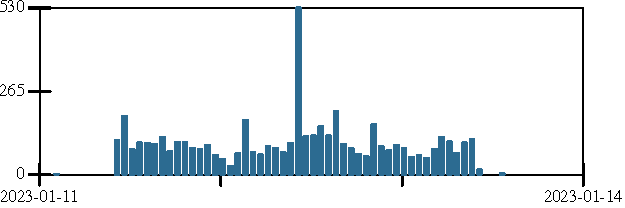
\includegraphics{img/row-distribution.pdf}
  \Description{FILL Histogram with approximately 100 records per hour, except for a 600-record spike near the end of Jan 12th.}
  \caption{Telemetry records per hour. Each tick on the $x$-axis marks the start of a new day in California.}
  \label{f:records-per-hour}
\end{figure}

\begin{figure}[t]
  TODO file size distribution: table or bars %% 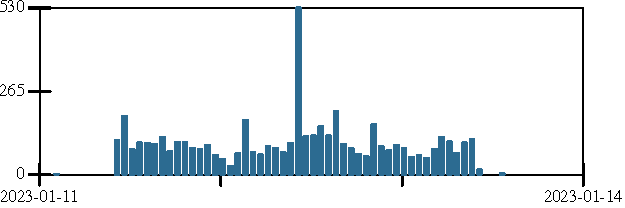
\includegraphics{img/row-distribution.pdf}
  \Description{FILL}
  \caption{Size of analyzed code: number of files, number of lines , and lines in edit region}
  \label{f:analysis-size}
\end{figure}


\Cref{f:records-per-hour} shows when data arrived across the whole dataset.
FILL: currently clientTimestamp, which has caveats.
Unclear what timezone they are from.
Some records have a client timestamp much older than the server, up to 1 week behind.
Some are ahead of the server by a day.
Why?
Could be wrong local settings on the computer, or a delayed record due to lost
internet connection or closed laptop.

\begin{figure}[t]
  \begin{tabular}{rl}
   5,001 & total logs \\
         & 4,471 \mnocheck{} + 506 \mnonstrict{} + 24 \mstrict{} \\
         & 1,628 from module switches \\
   182,247 & total forced strict type errors \\
         & {83,005 in module, 5,113 in edit regions} \\
    1,521 & total type errors \\
         & {1,035 in module, 110 non-syntax + 47 syntax in edit regions}
    \\[2ex]

    1,146 & sessions \\
    & \begin{tabular}{l}
      1,143 single mode = 1046 \mnocheck{} + 94 \mnonstrict{} + 3 \mstrict{} \\
        detected 2 multi-mode projects, 2 mode upgrades, 2 mode downgrades
      \end{tabular}
  \end{tabular}

  %% TODO these need to be plots, it's too much reading for the quick takeaway
  %% put exactly this data into bars!
  \begin{minipage}[t]{0.5\textwidth}
    \begin{tabular}{rr}
      Session length & \# Sessions \\\midrule
      1 &  450 \\
      2 &  199 \\
      3 &  129 \\
      4 &  73 \\
      5 &  60 \\
      6-10 & 150 \\
      11-20 & 67 \\
      21-40 & 11 \\
      >40 & 7
      %% max 393
    \end{tabular}
  \end{minipage}\begin{minipage}[t]{0.5\textwidth}
    \begin{tabular}{rr}
      Time delta & \# Records \\\midrule
      0-5ms & 284 \\
      5-1000ms & 248 \\
      1-2s & 153 \\
      2-5s & 232 \\
      5-10s & 207 \\
      10-30s & 524 \\
      30-60s & 392 \\
      1-2m & 394 \\
      2-5m & 559 \\
      5-10m & 360 \\
      >10-60m & 502
    \end{tabular}
  \end{minipage}

  \caption{Dataset overview}
  \label{f:dataset-overview}
\end{figure}

\begin{figure}[t]
  %% TODO stacked bars?
  %% TODO align old;curr
  \begin{tabular}{lrrrrr}
    Mode             & \# Rows & E         & Any Error & In Module & In Region \\
      & & & & (old ; curr) &  (old ; curr) \\\midrule
    \mnocheck{}   &   4,471 & \code{te} &    5.77\% &  0.20\% ;  2.21\% &  0.16\% ;  0.63\% \\
                  &         & \code{fs} &   59.18\% & 32.81\% ; 49.16\% &  9.17\% ; 13.13\% \\
    \mnonstrict{} &     506 & \code{te} &   25.89\% & 12.06\% ; 18.18\% &  6.32\% ;  7.91\% \\
                  &         & \code{fs} &   62.45\% & 37.94\% ; 53.75\% & 16.60\% ; 20.75\% \\
    \mstrict{}    &      24 & \code{te} &   50.00\% & 29.17\% ; 33.33\% &     0\% ;     0\% \\
                  &         & \code{fs} &   62.50\% & 50.00\% ; 58.33\% &  4.17\% ;  8.33\% 
  \end{tabular}

  \bigskip

  Below, edit region only.
  Each record with an edit region error adds +1 to at least 1 row.

  \smallskip

  %% TODO draw bars or curves b/c numbers are too hard to compare horizontally
  \begin{tabular}{lrrr}
    Error Label & \# Add & \# Keep & \# Remove \\\midrule
    CodeTooComplex
    & 0 & 0 & 0 \\
    UnificationTooComplex
    & 0 & 0 & 0 \\[1ex]
    SyntaxError
    & 30 & 0 & 76 \\
    UnknownSymbol
    & 12 & 14 & 19 \\
    UnknownProperty
    & 3 & 1 & 4 \\
    UnknownRequire
    & 1 & 5 & 0 \\
    GenericError
    & 1 & 0 & 1 \\
    CountMismatch
    &  1 &  0 &  1 \\
    OptionalValueAccess
    &  0 &  0 &  1 \\
  \end{tabular}

  \caption{Errors overview}
  \label{f:errors-overview}
\end{figure}

\Cref{f:dataset-overview}:
cannot filter syntax errors from the total and per-module error counts (\cref{s:threats});
multi-mode project = found a module switch that coincides with a mode switch, which suggests that two modules have different modes;
upgrade = found a up-mode switch that does not match a module switch (quite possible to miss these);
downgrade = found a down-mode switch that does not match a module switch

\begin{figure}[t]

  {Few local adds => Few people ignoring script analysis}
  \smallskip

  \begin{tabular}{lrrrr}
    & Local Remove & Local Add & Nonlocal Remove & Nonlocal Add \\
    Mode
    & \#err (\#log)
    & \#err (\#log)
    & \#err (\#log)
    & \#err (\#log) \\\midrule
    \mnocheck{}   & 86 (71) & 0 (0) & 110 (57) & 161 (74) \\
    \mnonstrict{} & 87 (25) & 9 (3) & 185 (29) & 207 (37) \\
    \mstrict{}    &  1  (1) & 0 (0) &  14  (6) &   6  (3) \\
  \end{tabular}

  \caption{Per-mode comparison}
  \label{f:mode-errors}
\end{figure}

\section{Interpretation}

\subsection{Code Too Complex}

The (example) code is NEVER too complex.


\subsection{TBD}

Error 1000 = type mismatch (subtyping etc);
1001 = unknown symbol;
\ldots

% https://github.com/Roblox/luau/blob/master/Analysis/include/Luau/Error.h


\begin{verbatim}
 require(foobar)
  foobar is a module script in the data model
 require(foo.bar.b)
  - could be edit in progress
  - could be renamed module
  - 
\end{verbatim}


\subsection{Module Switches}

FILL why study, what implications?

FILL need \%s out of all module switches.

How many module switches exit a module with errors?
\mnocheck{} 24, \mnonstrict{} 9, \mstrict{} 3.
Rare?
More common for forcedstrict:
 \mnocheck{} 190, \mnonstrict{} 16, \mstrict{} 2.

How many module switches go to a module with errors?
\mnocheck{} 70, nonstrict 9, strict 4
For FS: \mnocheck{} 400, \mnonstrict{} 39, \mstrict{} 6.


\subsection{Types and Quality of Life}

FILL error density: number vs region size

\begin{figure}[h]
  \begin{tabular}{llrrr}
    Mode & E & Add & Keep & Remove \\\midrule
    \mnocheck{}   & \code{te} & - & - & - \\
                  & \code{fs} & - & - & - \\
    \mnonstrict{} & \code{te} & 16 & 18 & 21 \\
                  & \code{fs} & 19 & 18 & 18 \\
    \mstrict{}    & \code{te} & - & - & - \\
                  & \code{fs} & - & - & - \\
  \end{tabular}

  \caption{Does mode influence the change in total error count?}
  \label{f:edit-deltas}
\end{figure}

TODO nocheck accumulated errors?


\subsection{Example Sessions}

FILL example sessions.

\Cref{f:ex-session-strict} begins in strict mode
but jumps to nocheck mode as well.
The jumps sometimes coincide with module switches (vertical line),
sometimes not.
The green line counts type errors.in the codebase.

\begin{figure}[t]
  \includegraphics[width=0.7\columnwidth]{img/example-session-strict.pdf}
  \caption{Example strict session}
  \label{f:ex-session-strict}
\end{figure}

\Cref{f:ex-session-nonstrict} presents the three sessions from \mnonstrict{} mode
that have the greatest number of events (not necessarily the longest time spans).
There are no module or mode switches.
There are few type errors.
One high point shows 10 errors, but these errors are gone (probably fixed) at
the next event.

\begin{figure}[t]
  \includegraphics[width=0.7\columnwidth]{img/example-session-nonstrict.pdf}
  \caption{Three most populated nonstrict sessions}
  \label{f:ex-session-nonstrict}
\end{figure}

\Cref{f:ex-session-nocheck} shows a roller coaster from \mnocheck{} mode.
Several hundred ForcedStrict type errors appear and disappear between events.
There are lots of module switches too \ldots but that makes no difference
for these project-wide error counts.

\begin{figure}[t]
  \includegraphics[width=0.7\columnwidth]{img/example-session-nocheck.pdf}
  \caption{Example nocheck session}
  \label{f:ex-session-nocheck}
\end{figure}


\subsection{Aggregate Sessions}

\begin{figure}[t]
  \includegraphics[width=0.8\columnwidth]{img/fit-nocheck-Force-3.pdf}
  \includegraphics[width=0.8\columnwidth]{img/fit-nonstrict-TypeE-3.pdf}
  \includegraphics[width=0.8\columnwidth]{img/fit-strict-TypeE-3.pdf}
  \caption{Best-fit curves for errors in each mode (\code{fs} for \mnocheck{}, \code{te} for the others)}
  \label{f:scribbles}
\end{figure}



\section{Threats to Validity}
\label{s:threats}

Error counts per-project and per-module include syntax errors.
Problematic, because syntax errors are uninteresting (easy to fix),
but common, which makes it likely that our per-keystroke telemetry will record them.
Edit region has specific counts.
Next time, we should do that for the other aggregates.


\section{Related Work}
\label{s:related}

\paragraph{Research on Errors}

Mind your language~\cite{mfk-onward-2011}.


\paragraph{Telemetry}

\begin{table}[t]
  \caption{Comparing telemetry systems}
  \label{t:telemetry-design}

  \begin{tabular}{l@{~}cccccc}
    &             & PII       & Session ID & Deterministic & Private Data \\\midrule
    & Transparent & \chkNo    & \chkNo     & \chkYes       & \chkNo      \\
  * & Lite        & \chkNo    & \chkYes    & \chkNo        & \chkYes     \\
    & \code{.NET} & \chkMaybe & \chkYes    & \chkYes       & \chkYes     \\
    & VS Code     & \chkYes   & \chkYes    & \chkYes       & \chkYes     \\
  \end{tabular}
\end{table}

Transparent telemetry: explain what it is and contrast our approach.
What essential, non-transparent things did we collect?

counting only, public decisions about what to count, public data,
collected weekly for a sample of clients, LastWeek field = prior day when
system gathered any data;
eg command invocations, lib stack frames, 
no user ID, no machine ID,
no time-ordered traces~\cite{transparent-telemetry}.

kindle track every tap (page turn etc),
enables whispersync feature,
drove design of navigation tools,
opt-out possible~\cite{kindle-telemetry}

vscode: usage data, crash reports, error data (not a crash but unexpected);
save file, open terminal, copy-paste, autocomplete offered, git queries, machine id,
session id, timestamp,
opt-out may be possible, but not for all usage data (per license, sec 2a) and
every extension can do its own thing~\cite{vscode-telemetry}

.NET SDK and .NET CLI:
crash reports, command invoked, args, hashed cwd, timings;
more listed online;
custom builds beware inadvertant disclosure, keep your filepaths clear;
data published in aggregate under CC-BY;
opt-out possible~\cite{dotnet-telemetry}




\section{Discussion}
\label{s:conclusion}
\label{s:discussion}



\begin{acks}
  TBD

Greenman was supported by
  \grantsponsor{NSF}{NSF}{https://www.nsf.gov} grant
 \href{"https://www.nsf.gov/awardsearch/showAward?AWD_ID=2030859"}{\grantnum{NSF}{CCF 2030859}}
  to the CRA for the \href{https://cifellows2020.org}{CIFellows} project.
\end{acks}

\bibliographystyle{ACM-Reference-Format}
\bibliography{bib}

\end{document}
\endinput
